\documentclass[11pt,letterpaper,boxed]{hmcpset}
\usepackage{fullpage}
\setlength{\parskip}{6pt}
\setlength{\parindent}{0pt}
\usepackage[margin=1in]{geometry}
\usepackage{graphicx}
\usepackage{enumerate}
\usepackage{marvosym}
\usepackage{amssymb}
\usepackage{wasysym}
\usepackage{gensymb}
\usepackage{mathrsfs}
\usepackage{scrextend}
\usepackage{mathtools}
\usepackage{pgfplots}
\usepackage{xspace}
\usepackage{esvect}
\usepackage{lipsum}
\usepackage{float}
\usepackage{esint}


\name{Name $\rule{4cm}{0.15mm}$}
\class{Physics 51M Section $\rule{.5cm}{0.15mm}$ Box \# $\rule{1cm}{0.15mm}$}
\assignment{Problem Set 8}
\duedate{11 November 2019}

\begin{document}
	
	%\begin{center}
	\noindent\textbf{Collaborators:} 
	%\end{center} 
	
	%\problemlist{}
	
	\begin{problem} [*HRK P32.6] Figure 32-40 shows an arrangement used to measure the masses of ions. An ion of mass $m$ and charge $+q$ is produced essentially at rest in source $S$, a chamber in which a gas discharge is taking place. The ion is accelerated by potential difference $\bigtriangleup V$ and allowed to enter a magnetic field $\vec{B}$. In the field it moves in a semicircle, striking a photographic plate at distance $x$ from the entry slit. Show that the ion mass $m$ is given by $m = \frac{B^2 q}{8\bigtriangleup V} x^2$.
		\begin{center}
		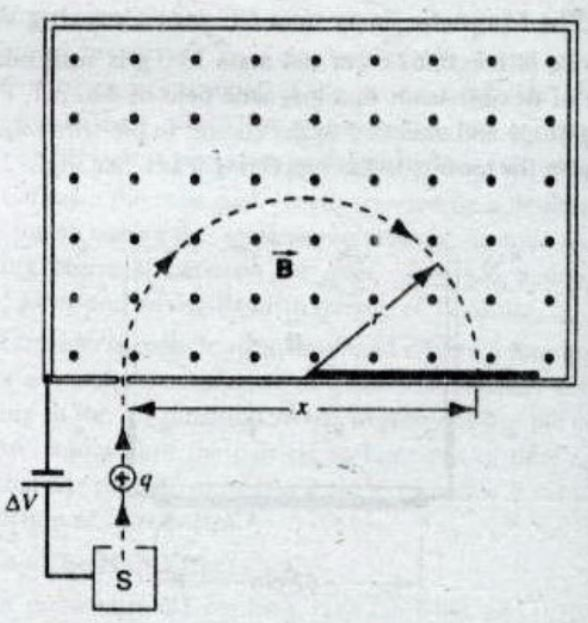
\includegraphics[scale=.2]{51m8pic.jpg}
		\end{center}
		
	\end{problem}
	
	\begin{solution}
		\vfill
	\end{solution}
	\newpage

	\begin{problem} [HRK E33.13] Consider the circuit of Fig. 33-42. The curved segments are along the radii. Find the magnetic field $\vec{B}$ at $P$, assuming a current $i$ in the circuit.
	\begin{center}
		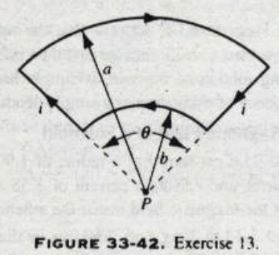
\includegraphics[scale=.5]{51m8pic2.jpg}
		\end{center}
	\end{problem}
	\begin{solution}
		\vfill
	\end{solution}
	\newpage

	\begin{problem} [HRK E33.15] Figure 33-43 shows a cross section of a long, thin ribbon of width $w$ that is carrying a uniformly distributed total current $i$ into the page. Calculate the magnitude and the direction of the electric field $\vec{B}$ at a point $P$ in the plane of the ribbon at a distance $d$ from its edge. (Hint: Imagine the ribbon to be constructed from many long, thin, parallel wires.)
			\begin{center}
		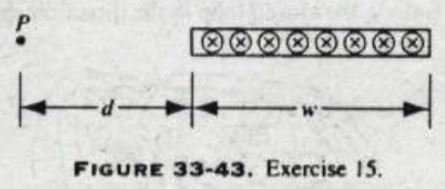
\includegraphics[scale=.5]{51m8pic3.jpg}
		\end{center}
	\end{problem}
	
	\begin{solution}
		\vfill
	\end{solution}
	\newpage	
	
	\begin{problem}[HRK E33.24] Figure 33-50 shows a long wire carrying a current $i_2$. Calculate the resultant force acting on the loop. Assume that $a = 1.10 cm, b = 9.20 cm, L = 32.3 cm, i_1 = 28.6 A$, and $i_2 = 21.8A$.
				\begin{center}
		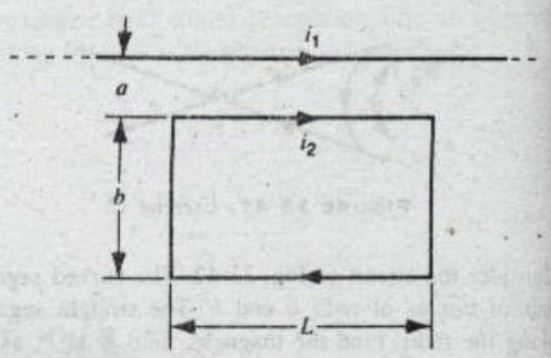
\includegraphics[scale=.3]{51m8pic4.jpg}
		\end{center}
	\end{problem}
	
	\begin{solution}
		\vfill
	\end{solution}
	\newpage
	
	\begin{problem}A conductor consists of an infinite number of adjacent wires, each infinitely long and carrying a current $i$. Show that the lines of $\vec{B}$ are as represented in the figure and that $B$ for all points above and below the infinite current sheet is given by $B = \frac{1}{2} \mu_0 ni$, where $n$ is the number of wires per unit length.
	\begin{center}
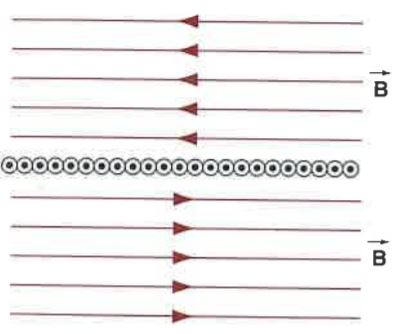
\includegraphics[scale=.3]{51m8pic5.jpg}
\end{center}		
	\end{problem}
	
	\begin{solution}
		\vfill
	\end{solution}
	\newpage
	
	\begin{problem}[HRK P33.13] The current density inside a long, solid, cylindrical wire of radius $a$ is in the direction of the axis and varies linearly with radial distance $r$ from the axis according to $j = \frac{j_0 r}{a}$. Find the magnetic field inside the wire. Express your answer in terms of the total current $i$ carried by the wire.
	\end{problem}
	
	\begin{solution}
		\vfill
	\end{solution}
	\newpage
	
	
\end{document}
